\textbf{2-1} 如电图2-1-1所示，电流强度为 $2I$ 的直流电经半无限长导线到达半径为 $R$ 的金属球面的南极点，由球面流到北极点后，再从另一半无限长直导线流向远处。设想将上述电流分布切成左、右两半。左半部分为半无限长直电流 $I$ 到达半球面南极点后，经左半球面（注意，此半球面的电流分布与原全球面左半的电流分布相同）流向北极点，再经半无限长直导线流向远处，并设置 $O - xyz$ 坐标，如图2-1-2所示。试求球心 $O$ 处的磁感应强度 $\pmb{B}$

\begin{center}
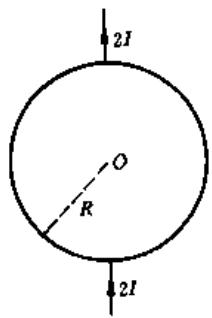
\includegraphics[width=0.15\textwidth]{figures/电图2-1-1.jpg}
\qquad
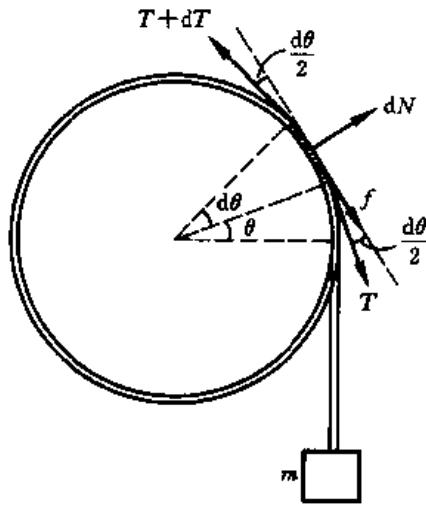
\includegraphics[width=0.2\textwidth]{figures/图2-1-2.jpg}
\end{center}
\vfill

\textbf{2-2} 抛物线形状的无穷长导线载有电流 $I$ 。设焦点到顶点的距离为 $a$ 。试求焦点处的磁感应强度 $B$ 。
\vfill

\newpage
\textbf{2-3} 均匀带电的球面绕着它的某一直径匀速旋转．试证明在该直径上的磁感应强度处处相同．
\vfill

\textbf{2-4} 如电图2-4-1所示，在Oxyz坐标系中有一半径为R的无限长圆柱面，圆柱面的中央轴线沿y轴，圆柱面上绕有螺距为H的无限长等距螺旋导线，导线与x轴相交，导线内通有稳恒电流I.设空间各处的相对磁导率近似为1，试求坐标原点O处的磁感应强度B的三个直角坐标分量 $B_{x},B_{y}$ 和 $B_{z}$ .

\begin{center}
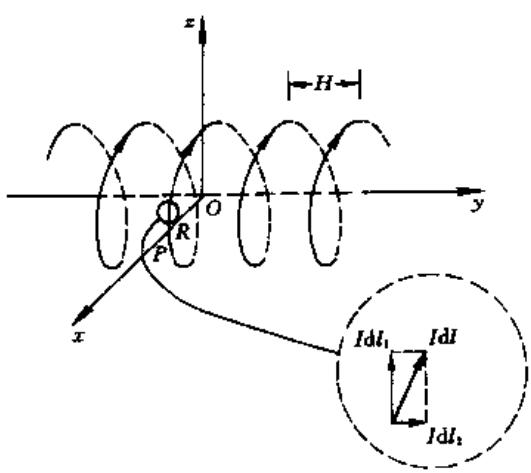
\includegraphics[width=0.3\textwidth]{figures/电图2-4-1.jpg}
\end{center}
\vfill

\newpage
\textbf{2-5} 如电图2-5-1， $C_{+}$ 和 $C_{-}$ 是沿 z 轴放置的两根互相绝缘的长直非磁性导体，其中的电流分别沿 z 轴的正方向和负方向流动, 电流强度均为 $I$ 。图中画斜线的部分是两导体的正截面, 它们分别是 $xy$ 平面中的部分圆, 两圆的直径均为 $D$ , 两圆心的间距为 $\frac{D}{2}$ , 不难算出, 两导体正截面的面积均为 $\left(\frac{1}{12}\pi + \frac{1}{8}\sqrt{3}\right) D^2$ 。每一根导体中的电流均匀地分布在自身的正截面内。 试求两根导体之间空白区域内的磁场分布 $B(x, y)$ 。

\begin{center}
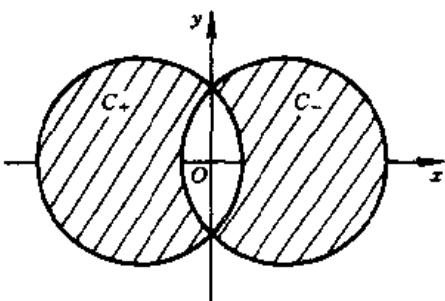
\includegraphics[width=0.25\textwidth]{figures/电图2-5-1.jpg}
\end{center}
\vfill

\textbf{2-6} 如电图2-6-1所示，取直角坐标系 $xyz$ ，在 $-d\leqslant x\leqslant d$ 的一层无穷区域内有均匀的传导电流，电流密度的方向为 $z$ 轴的正方向，大小恒定为 $j$ 试求真空中磁感应强度 $\pmb{B}$ 的分布。

\begin{center}
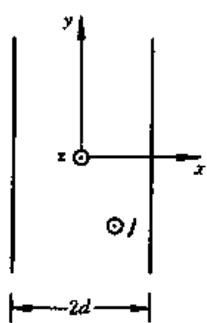
\includegraphics[width=0.25\textwidth]{figures/电图2-6-1.jpg}
\end{center}
\vfill

\newpage
\textbf{2-7} 无限长直圆柱形导体在没有电流时，自由电子的体电荷密度为常量 $\rho_0$ ，正离子的体电荷密度为 $-\rho_0$ ，导体内处于电中性。当沿导体长度方向通以直流电时，体电流会在导体中产生轴对称的环状分布磁场，沿轴向运动的自由电子便会在磁场力的作用下向中轴移动，从而破坏了原来的 $\rho_0$ 分布。当积聚的净电荷产生的径向电场与运动自由电子所受的磁场力恰好抵消时，便形成只沿导体长度方向的稳恒电流。设此时自由电子的漂移速度为 $\bar{u}$ 。试求导体中净电荷密度的分布。
\vfill  

\textbf{2-8} 如电图2-8-1，在水平面上有一根光滑的刚性细长杆，它可以无摩擦地绕固定的竖直轴旋转，转动惯量为 $I$ 。在杆周围有与转轴平行的匀强磁场 $\pmb{B}$ ，其方向如图所示。把质量为 $m$ ，电量为 $q(q>0)$ 的光滑带电小圆环套在杆上,设环与杆之间无电荷转移。

1. 试问杆连同环的旋转角速度 $\omega$ 取何值时, 环在杆上任何位置均可相对杆静止。

2. 设杆的初始角速度 $\omega_{0}$ 大于第 1 问中的 $\omega$ 值，设开始时环静止于转轴位置，后因受微小扰动，环离开转轴位置沿杆运动。试问环是否可能在到达杆的某一位置后，其径向速度降为零，从而停留在该处相对杆保持静止。

3. 若杆的初始角速度改取第2问中所给初始角速度的 $\alpha$ 倍 $(\alpha > 0)$ . 试问为使圆环的运动轨道保持不变, 应如何改变磁场的大小。

\begin{center}
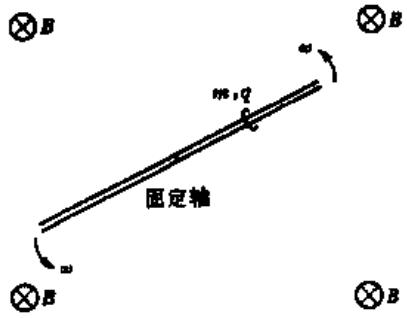
\includegraphics[width=0.2\textwidth]{figures/电图2-8-1.jpg}
\end{center}
\vfill

\newpage
\textbf{2-9} 如电图2-9-1所示，半径为 $R$ ，质量为 $m$ 的匀质细圆环上均匀地分布着相对圆环固定不动的正电荷，总电量为 $Q, t = 0$ 时，圆环在水平地面上具有沿正东方向的平动速度 $\nu_{0}$ ，且无滚动．假设圆环与地面之间的摩擦系数为 $\mu$ ，在圆环周围只有沿水平面指向北方（电图 2-9-1 中垂直纸面向里为北方）的匀强地磁场 B．

1. 为了使圆环在尔后的运动过程中始终不会离开地面，试求 $v_{0}$ 的取值范围。

2. 若 $v_{0}$ 在第一问的取值范围内, 假设圆环最后能达到纯滚状态. 试导出在达到纯滚前, 圆环的平动速度 $v$ 与时间 $t$ 的关系。

3. 设 $v_{0}=\frac{mg}{2QB}$ ，试求圆环则达到纯滚状态的时刻 T.

\begin{center}
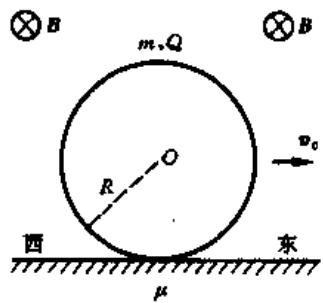
\includegraphics[width=0.2\textwidth]{figures/电图2-9-1.jpg}
\end{center}
\vfill

\textbf{2-10} 如电图2-10-1所示，经 $U = 1000\mathrm{V}$ 电压加速的电子(加速前电子静止)从电子枪T射出，其初速沿直线 $\alpha$ 的方向。若要求电子能击中在 $\varphi = 60^{\circ}$ 方向，与枪口相距 $d = 5.0~\mathrm{cm}$ 的靶M。试求在以下两种情形，所需的匀强磁场的磁感应强度 $\pmb{B}$ 的大小。1. 磁场 $\pmb{B}$ 垂直于直线 $\alpha$ 与靶 M 所确定的平面.2. 磁场 B 平行于枪口 T 向靶 M 所引的直线 TM.

\begin{center}
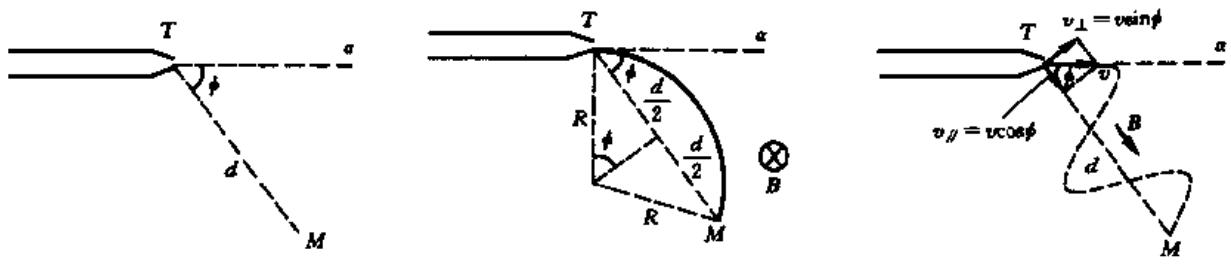
\includegraphics[width=0.6\textwidth]{figures/电图2-10-1.jpg}
\end{center}
\vfill

\newpage
\textbf{2-11} 如电图2-11-1所示，设在本题所涉及的空间范围内有磁感应强度为 $\pmb{B}$ 的匀强磁场，其方向垂直纸平面向里。在纸平面上有一个长为 $h$ 的光滑绝缘空心细管MN，在管的 $M$ 端内有一个质量为 $m$ ，电量为 $q(q > 0)$ 的带电小球 $\mathbf{P}_1$ ，在管的 $N$ 端外侧有另一个不带电的小球 $\mathbf{P}_2$ 。开始时， $\mathbf{P}_1$ 相对管静止，管带着 $\mathbf{P}_1$ 以垂直于管长度方向的速度 $\pmb{u}_{1}$ 在纸面上向图中正右方向运动，小球则以 $\pmb{u}_{2}$ 向着图中正左方向运动。设管的质量远大于 $m$ ，小球 $\mathbf{P}_1$ 在管内运动对管运动的影响可以忽略。设引力可略。如果 $\mathbf{P}_1$ 从管的 $N$ 端离开管后，最终能与 $\mathbf{P}_2$ 相碰。试求满足此要求的 $\pmb{u}_{2}$ 的可能取值。

\begin{center}
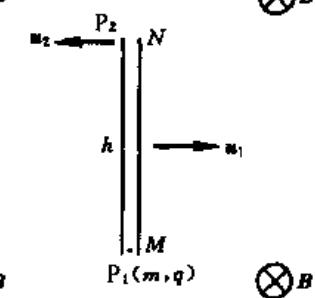
\includegraphics[width=0.2\textwidth]{figures/电图2-11-1.jpg}
\end{center}
\vfill
\newpage

\textbf{2-12} 如电图2-12-1所示，在半径为 $R$ 的圆筒形真空管中有两个隔板，将管内分为三个区域，两隔板中心各有小孔A和 $\mathbf{A}^{\prime}$ ，两孔间距为 $L$ 。在左边的区域I中有加速电场，在中间的区域Ⅱ中有沿管轴方向的匀强磁场 $\pmb{B}$ ，在右边的区域Ⅲ中既无电场也无磁场。区域I中的阴极K连续发射的电子经其中的电场加速后，使穿过小孔A的电子形成发散束进入区域II。设穿过小孔A的这些电子的速度在管轴方向的分量均为 $v$ ，设电子之间的相互作用可以忽略。当将区域Ⅱ中沿管轴方向的磁感应强度的大小调到某些值时，从小孔A进入区域Ⅱ的电子便能穿过小孔 $\mathbf{A}^{\prime}$ 射出，把这些磁场的最小值表为 $B_{0}$ 。取从A到 $\mathbf{A}^{\prime}$ 的方向为正方向，区域Ⅱ中的磁场 $\pmb{B}$ 随时间 $t$ 变化的曲线如电图2-12-2所示。即从 $t = 0$ 起 $\pmb{B}$ 沿正方向，每经 $\frac{T}{2}$ 的时间 $\pmb{B}$ 反向一次， $T$ 就是 $\pmb{B}$ 的变化周期。从 $t = 0$ 开始，电子束连续地从小孔A进入区域Ⅱ，设凡遇管壁的电子均被管壁吸收。

1. 为了使从小孔 A 进入区域 II 的电子能经小孔 A' 到达区域 III, 试求磁场 B 变化周期的最小值 $T_{0}$ .

2. 若取磁场变化周期 $T = 2T_0$ ，试在电图 2-12-2 的时间轴上标明电子能经小孔 A' 到达区域Ⅲ的时间区间。

3. 在进入区域Ⅲ的电子束中, 电子运动方向与管轴之间夹角的最大值是多少?

\begin{center}
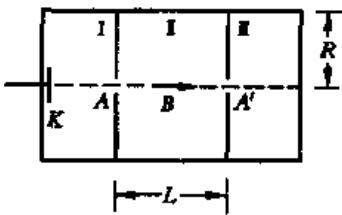
\includegraphics[width=0.3\textwidth]{figures/电图2-12-2.jpg}
\quad
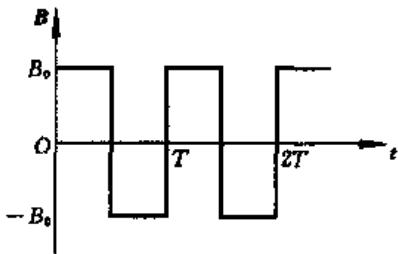
\includegraphics[width=0.3\textwidth]{figures/电图2-12-1.jpg}
\end{center}

\vfill

\newpage
\textbf{2-13} 如电图2-13-1所示，一个实心圆柱形导体和一个中空圆柱形导体共轴，其间为真空，内圆柱体的半径为 $a$ ，外圆柱体的内半径为 $b$ 。外圆柱体相对内圆柱体可具有正电势 $V$ ，故称为阳极．在涉及的空间范围内可以存在匀强磁场，磁感应强度 B 的方向与圆柱体的中央轴平行，即垂直于电图 2-13-1 所在的纸平面并外指．设导体的感应电荷一律不予考虑。

本题讨论电子在两圆柱体之间的真空中运动的动力学问题。设电子的静止质量为 m，电量为 -e，电子一律从内圆柱体表面射出。

1.设外圆柱体相对内圆柱体的电势为 $V$ , 设 $B = 0$ . 设有一个电子从内圆柱体表面逸出, 初速可略。试求该电子打到阳极 (外圆柱体) 时的速度大小为 $v$ , 先给出非相对论的答案, 再给出相对论的答案.

以下几问则无需考虑相对论效应。

2.设 $V = 0$ , 设匀强磁场 $\pmb{B}$ 不为零。一个电子以径向初速度 $\nu_0$ 从内圆柱体表面射出, 当磁场超过某一临界值 $B_{\mathrm{C}}$ 时, 电子将不能到达阳极 (外圆柱体), 试求此 $B_{\mathrm{C}}$ 值, 并在磁场略大于 $B_{\mathrm{C}}$ 的情况下, 定性画出电子与内圆柱体相碰前的运动轨道。

3.电子从内圆柱体射出后, 磁场对电子的作用可使电子获得相对圆柱体中央轴的非零角动量 $L$ . 试导出 $L$ 随时间 $t$ 的变化率 $\frac{\mathrm{d}L}{\mathrm{d}t}$ 的表达式。试进而证明, 这一表达式意味着下述量
$$
L - k e B r ^ {2}
$$
是一个不随电子运动而变化的守恒量．其中 k 是一个无量纲的常量，r 是从圆柱体中央轴到电子所在位置的矢径．最后，试确定 k 的值．

4.设一个电子无初速地从内圆柱体表面逸出后不能到达阳极，则它与圆柱体中央轴的距离必定会达到某个相应的极大值 $r_{\max}$ 。试求电子到达该 $r_{\max}$ 距离的速度大小 $v$ 与 $r_{\max}$ 的关系。

5.若感兴趣的是如何利用磁场 B 来限制到达阳极的电子流。设当 B 稍大于某个临界值 $B_{C}$ 时，从内圆柱体表面无初速地逸出的电子便不能到达阳极。试确定此 $B_{C}$ 值。

6.加热内圆柱体, 使电子从内圆柱表面逸出时具有非零的初速度。设电子初速度沿 B 方向的分量为 $v_{B}$ , 沿径向向外的分量为 $v_{r}$ , 逆时针的角向分量为 $v_{\phi}$ . 对于这种情形, 试求刚好能使电子到达阳极的临界磁场 $B_{C}$ .

\begin{center}
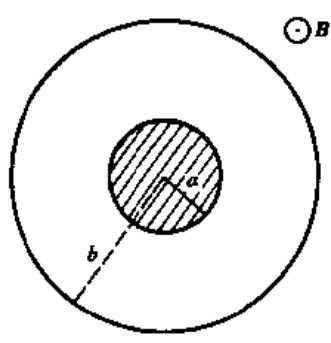
\includegraphics[width=0.2\textwidth]{figures/电图2-13-1.jpg}
\end{center}
\vfill
\newpage

\textbf{2-14} 如电图2-14-1所示，一簇质量均为 $m$ ，电量均为 $q$ 的离子在 $P$ 点以同一速率 $\pmb{v}$ 沿 $xy$ 上半平面中的各个方向射出．垂直于 $xy$ 平面的均匀磁场 $B$ 将这些离子聚焦在 $R$ 点， $P$ 点与 $R$ 点相距为 $2a$ ，离子的轨道应是轴对称的．试确定磁场区的边界．设离子之间的相互作用可以忽略。

\begin{center}
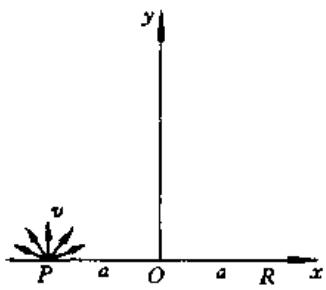
\includegraphics[width=0.2\textwidth]{figures/电图2-14-1.jpg}
\end{center}
\vfill


\textbf{2-15} 如电图2-15-1所示，在 $xy$ 平面上有一束稀疏的电子(其间的相互作用可以忽略)，在 $-H < y < H$ 范围内，从 $x$ 负半轴的远处以相同的速率 $v$ 沿着 $x$ 轴方向平行地向 $y$ 轴射来.

试设计一磁场区,使得

1.所有电子都能在磁场力的作用下通过坐标原点O.

2.这一片电子最后扩展到-2H<y<2H范围内继续沿着x轴方向向x正半轴的远处平行地以相同速率v射去.

\begin{center}
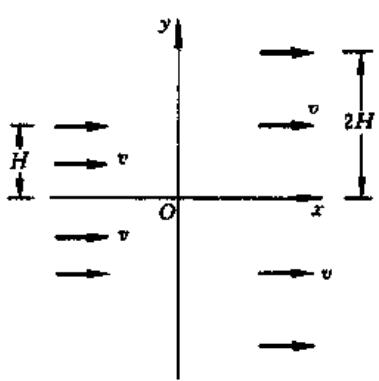
\includegraphics[width=0.2\textwidth]{figures/电图2-15-1.jpg}
\end{center}
\vfill
